\documentclass[11pt]{article}

\usepackage{graphicx}
\usepackage{caption}
\usepackage{subcaption}

\begin{document}

\centerline{\Large\bf Figures Example}\par
\bigskip

\section{Single Figure}

Insert a figure with a caption and label, then reference it like Figure \ref{fig:single}.

\begin{figure}[h!]
	\centering
	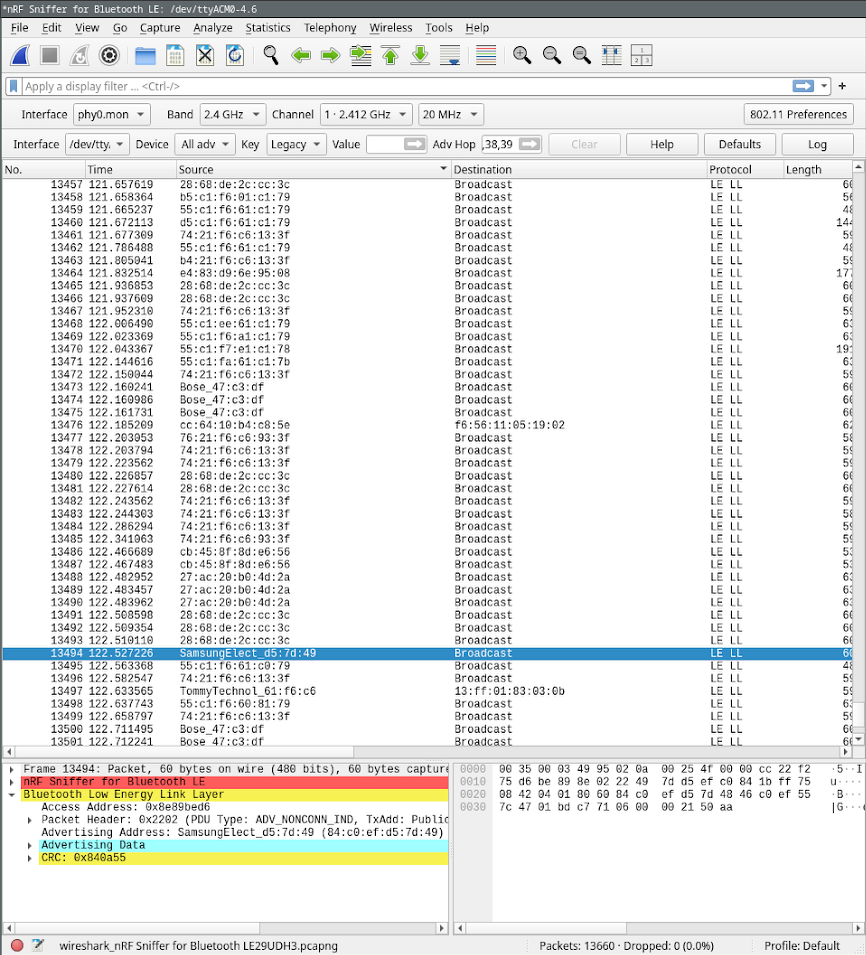
\includegraphics[width=0.8\textwidth]{assets/ble_noise.png}
	\caption{A single figure with a caption.}
	\label{fig:single}
\end{figure}

\section{Side-by-Side Figures}

Two figures side by side using \texttt{minipage}:

\begin{figure}[h!]
	\centering
	\begin{minipage}{0.45\textwidth}
		\centering
		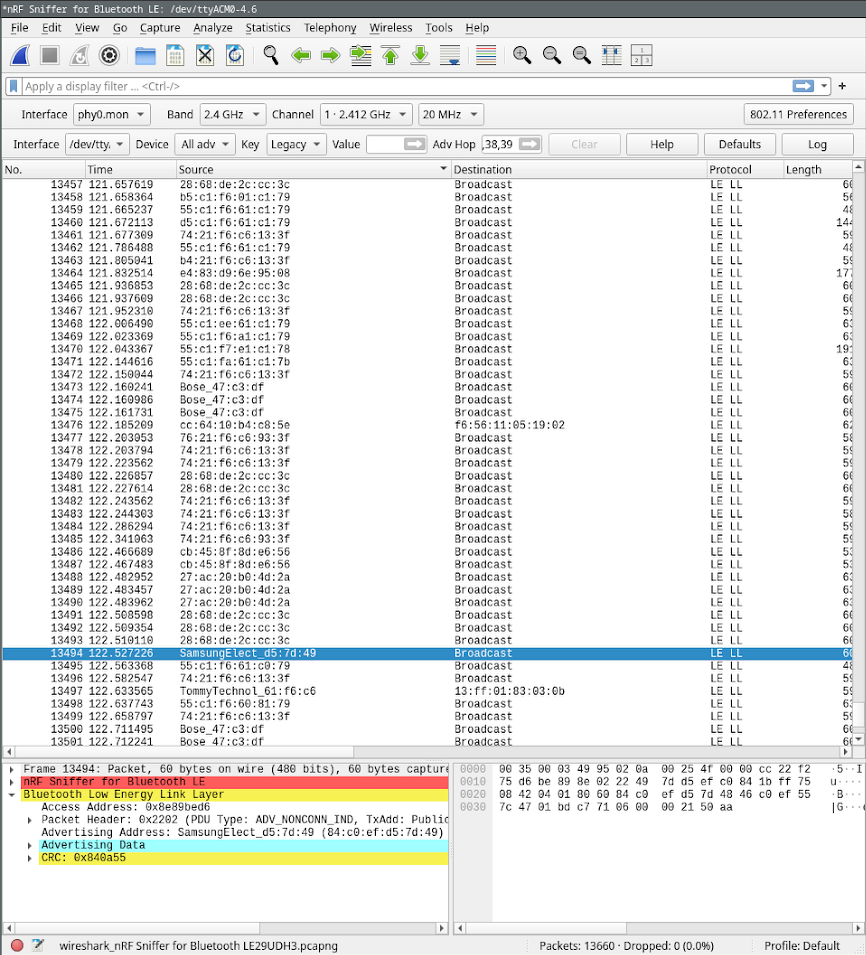
\includegraphics[width=\textwidth]{assets/ble_noise.png}
		\caption{Left figure.}
		\label{fig:left}
	\end{minipage}
	\hfill
	\begin{minipage}{0.45\textwidth}
		\centering
		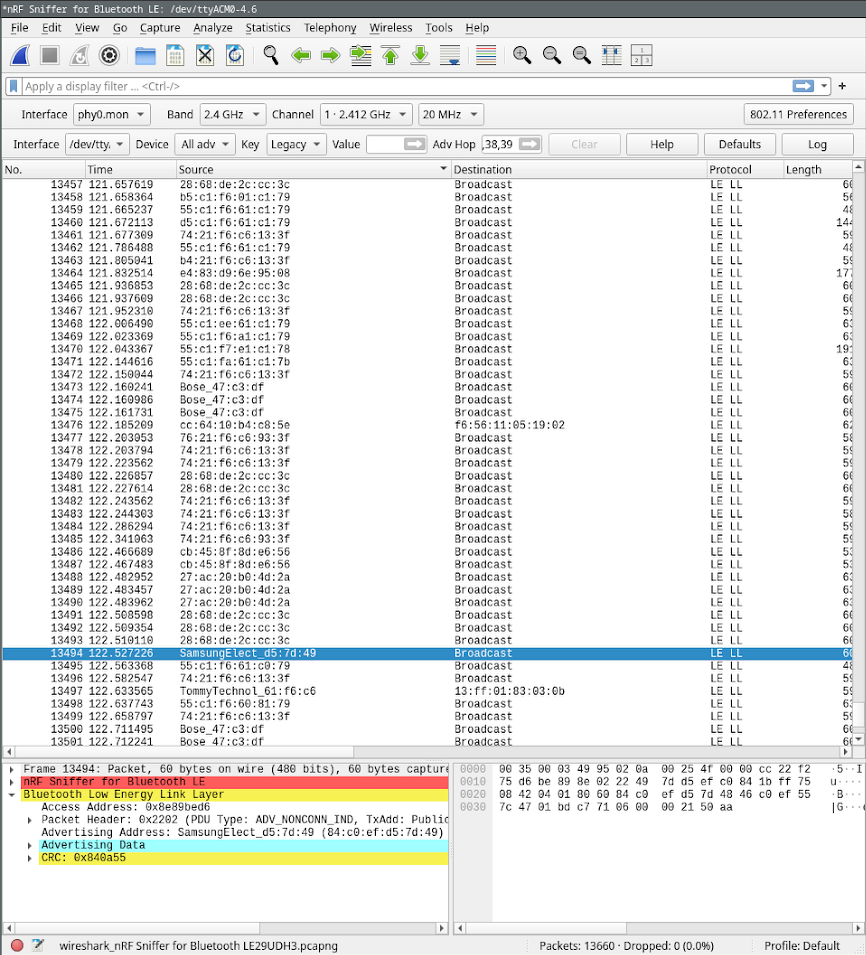
\includegraphics[width=\textwidth]{assets/ble_noise.png}
		\caption{Right figure.}
		\label{fig:right}
	\end{minipage}
\end{figure}

\section{Subfigures}

Two subfigures under a shared caption using \texttt{subcaption}, referencing Figure \ref{fig:sub}
(or individually as Figure \ref{fig:sub-a} and Figure \ref{fig:sub-b}):

\begin{figure}[h!]
	\centering
	\begin{subfigure}{0.45\textwidth}
		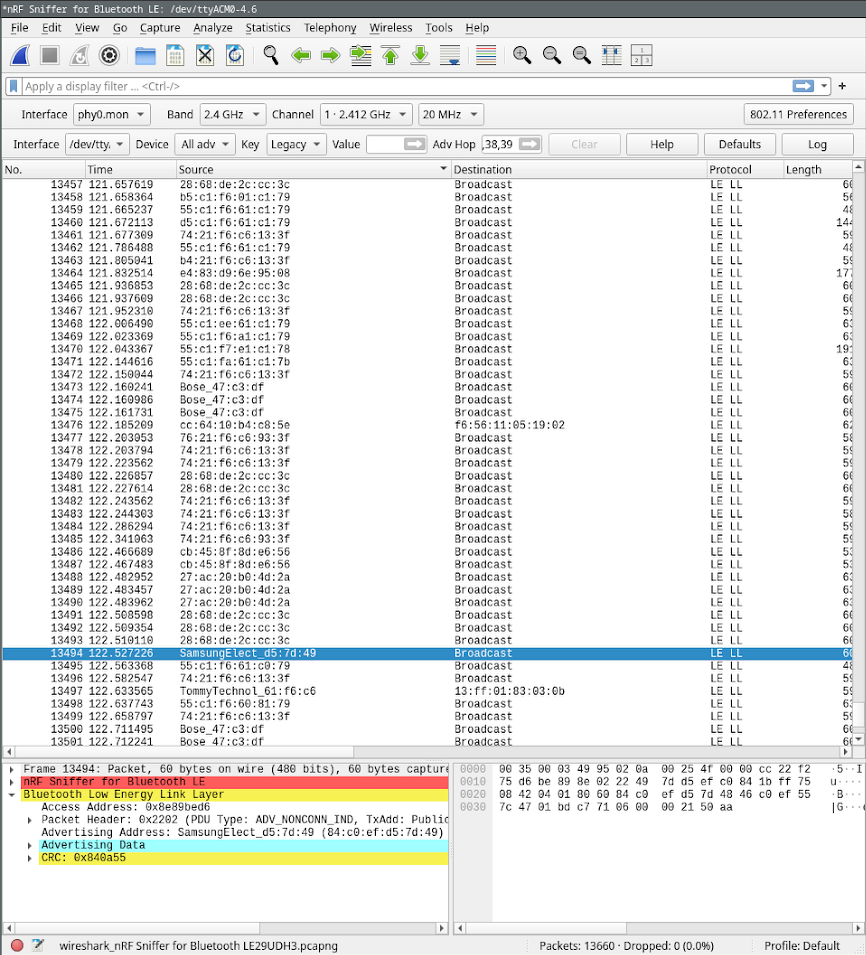
\includegraphics[width=\textwidth]{assets/ble_noise.png}
		\caption{Subfigure A.}
		\label{fig:sub-a}
	\end{subfigure}
	\hfill
	\begin{subfigure}{0.45\textwidth}
		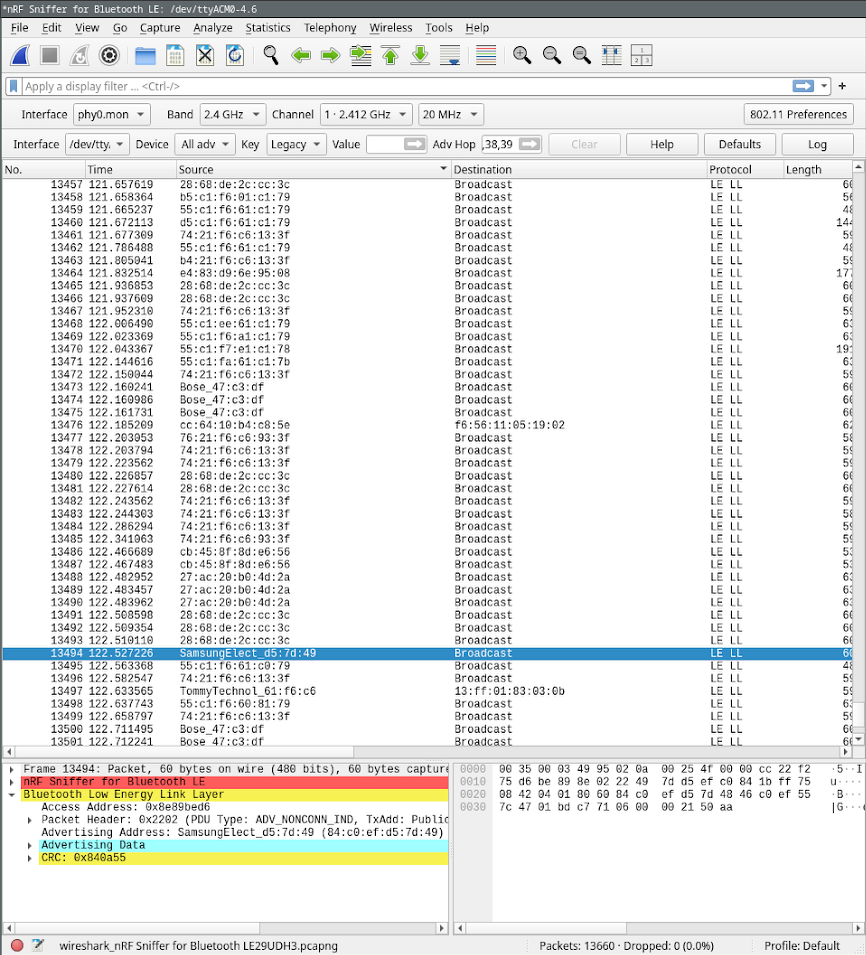
\includegraphics[width=\textwidth]{assets/ble_noise.png}
		\caption{Subfigure B.}
		\label{fig:sub-b}
	\end{subfigure}
	\caption{Two subfigures with a shared caption.}
	\label{fig:sub}
\end{figure}

\end{document}
